\documentclass[12pt]{article}
\usepackage{amsmath}
\usepackage[pdftex]{graphicx}
\usepackage{natbib}
\usepackage[margin=1in]{geometry}

%% make lists more compact
\usepackage{enumitem}
\setitemize{noitemsep,topsep=0pt,parsep=0pt,partopsep=0pt}
\setenumerate{noitemsep,topsep=0pt,parsep=0pt,partopsep=0pt}

\title{Supplement to ``Community assembly on isolated islands:
  Macroecology meets evolution''}

\author{}

\date{}

%%%%%%%%%%%%%%%%% END OF PREAMBLE %%%%%%%%%%%%%%%%

\begin{document}
\baselineskip24pt
\maketitle

A. J. Rominger$^{1*}$,
K. R. Goodman$^{1*}$, 
J. Y. Lim$^{2*}$, 
E. Armstrong$^{1,3+}$,
L. E. Becking$^{1,4}$
G. M Bennett$^5$,
M. S. Brewer$^{1,6+}$, 
D. D. Cotoras$^{2,7+}$, 
C. P. Ewing$^3$, 
J. Harte$^1$,
N. Martinez$^8$,
P. O’Grady$^1$,
D. Percy$^9$,
D. Price$^3$,
G. K. Roderick$^1$,
K. Shaw$^10$,
F. S. Valdovinos$^{8*}$, 
D. S. Gruner$^{11\#}$,
R. G. Gillespie$^{1\#}$

\vspace{1em}

\begin{enumerate}
\item Department of Environmental Science, Policy, and Management, University of
  California, Berkeley, California 94720-3114
\item Department of Integrative Biology, University of California, Berkeley,
  California 94720-3140
\item Department of Biology, University of Hawaii, Hilo, Hawaii, 96720-4091
\item Department of Integrative Biology, University of Texas, Austin, Texas 78712
\item Department of Entomology, The Natural History Museum, London, UK SW7 5BD
\item Pacific Ecoinformatics and Computational Ecology Lab, Berkeley,
  California 94703
\item Department of Neurobiology and Behavior, Cornell, Ithaca, New York 14853-7601
\item Department of Entomology, University of Maryland, College Park,
  Maryland 20742-4454
\item[*] Contributed equally;
\item[+] Current affiliation;
\item[\#] co-senior authors; 
\item[] corresponding author: R. G. Gillespie, gillespie@berkeley.edu.
\end{enumerate}

\clearpage


\section{Compilation of networks and metric validation}

We compiled plant-herbivore networks from published sources as
described in the main text.  Table \ref{tab:networkPubs} lists
publications used in compiling these networks.

Researchers have put forward to set of ``network metrics,'' including
nestedness \citep{Bascompte2003, Ulrich2009} and modularity
\citep{Newman2004, Olesen2007}, to understand the complex structure of
ecological networks. Null models are used to evaluate the statistical
significance of these metrics and to compare between networks of
different size \cite{Ulrich2009}. We compare the results derived from
two common null models: the ``probabilistic null'' of
\cite{Bascompte2003} using the relative degree distributions of plants
and herbivores as weights while randomizing links and suffers from
high Type II error \citep{Ulrich2009}; the ``fixed-fixed null''
\citep{Ulrich2009} maintains the exact number of links assigned to
each species while randomizing which interactors fill the requisite set
of links and suffers from high Type I error \citep{Ulrich2009}. We find that
using these different null models does not change any trends in our
network statistics across the Hawaiian chronosequence but different
null models do influence the sign and significance of the network
metrics (Fig. \ref{figSupp:netMetComp}). We therefore do not interpret
the sing or significance of the metrics but only their relative trends
across site age.

Because these networks are based on opportunistic data associated with
species descriptions, and not based on standardized ecological
surveys, we cannot interpret patterns in network metrics without
evaluating possible sampling biases \citep{Nielsen2007, Gibson2011,
  Rivera2012}.  To do so we rarify networks by the number of Hemiptera
species included and, for each subsampled network, re-calculate
nestedness and modularity z-scores. This rarefaction procedure shows
that nestedness is very sensitive to network size
(Fig. \ref{figSupp:rfy}), a known property of nestedness
\citep{Nielsen2007, Gibson2011, Rivera2012}. However the relative
nestedness z-scores across networks remain qualitatively similar to
those observed for the complete networks (Fig. \ref{figSupp:rfy}).
Modularity depends on network size in a more variable way
(Fig. \ref{figSupp:rfy}). Modularity is expected to decrease with
network size \citep{Rivera2012} and so the marked increase in
modularity with network size on Haleakala is unexpected. However in
light of the large number of highly specialized taxa this pattern is
more reasonable---if most species only have within module links then
removing these species through subsampling will only reduce overall
modularity.  Thus this pattern speaks to the high level of
specialization on Haleakala, and to a lesser extent at Kokee which
also shows a slight increase in modularity with network size
(Fig. \ref{figSupp:rfy}).

\bibliographystyle{geb}
\bibliography{dimensions_geb}

\clearpage

\section{Supplemental Figures}

\begin{figure}[!hp]
  \centering
  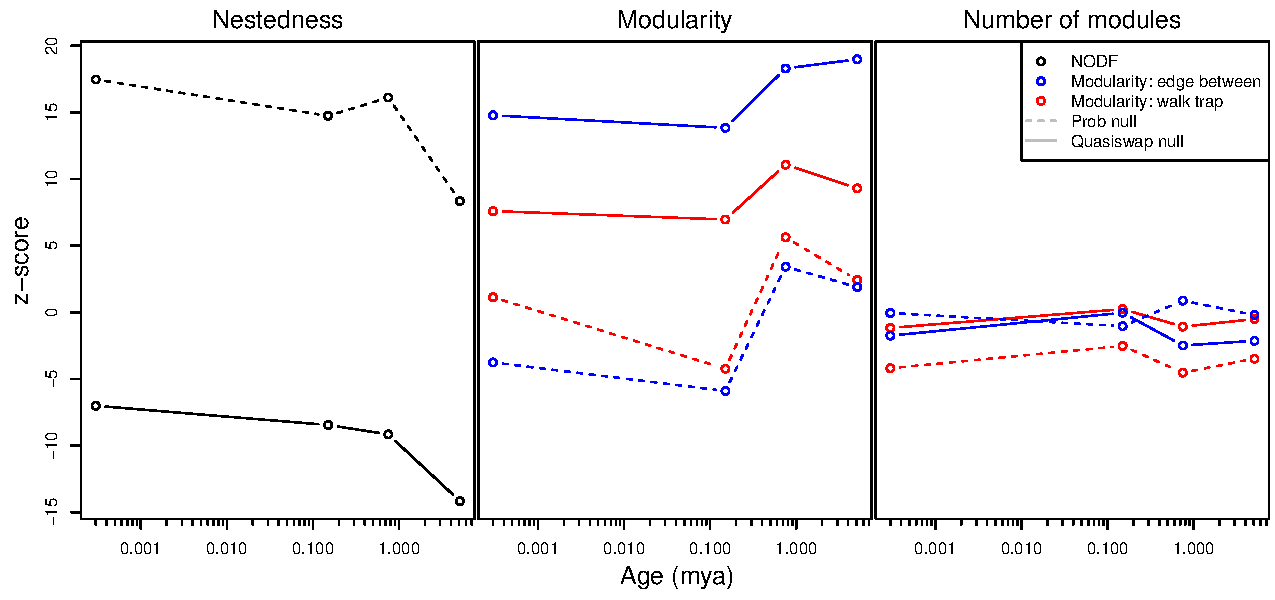
\includegraphics[scale=0.6]{../figSupp_netMetComp.pdf}
  \caption{Comparison of different null models (``Prob'' and
    ``Quasiswap'') used to standardize network metrics and comparison
    of different algorithms for assessing modularity (``edge between''
    and ``walk drap''). Choice of null model has a strong influence
    on the sign and magnitude of metrics but not on their relative
    trends. The different modularity algorithms lead to largely
    similar qualitative patterns.}
  \label{figSupp:netMetComp}
\end{figure}

\begin{figure}[!hp]
  \centering
  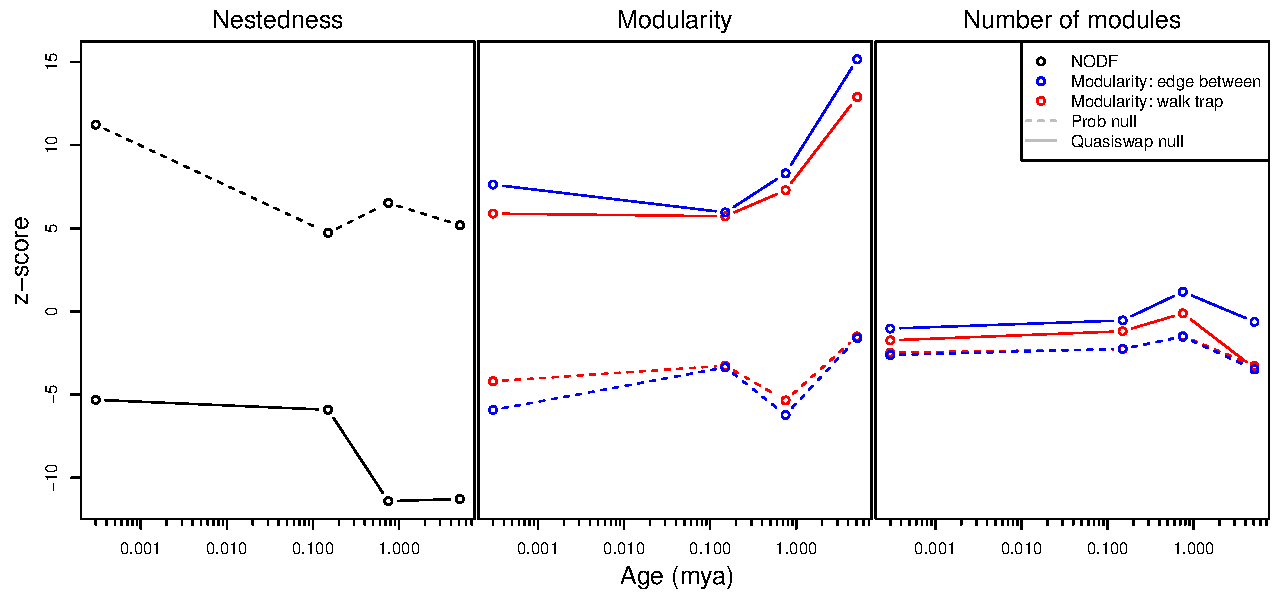
\includegraphics[scale=0.6]{../figSupp_netMetCons.pdf}
  \caption{Metrics NODF and modularity calculated for networks based
    on more biogeographically conservative assignment of Hemiptera to
    localities. Colors and metric specifics as in Figure
    \ref{figSupp:netMetComp}.}
  \label{figSupp:netCons}
\end{figure}

\begin{figure}[!hp]
  \centering
  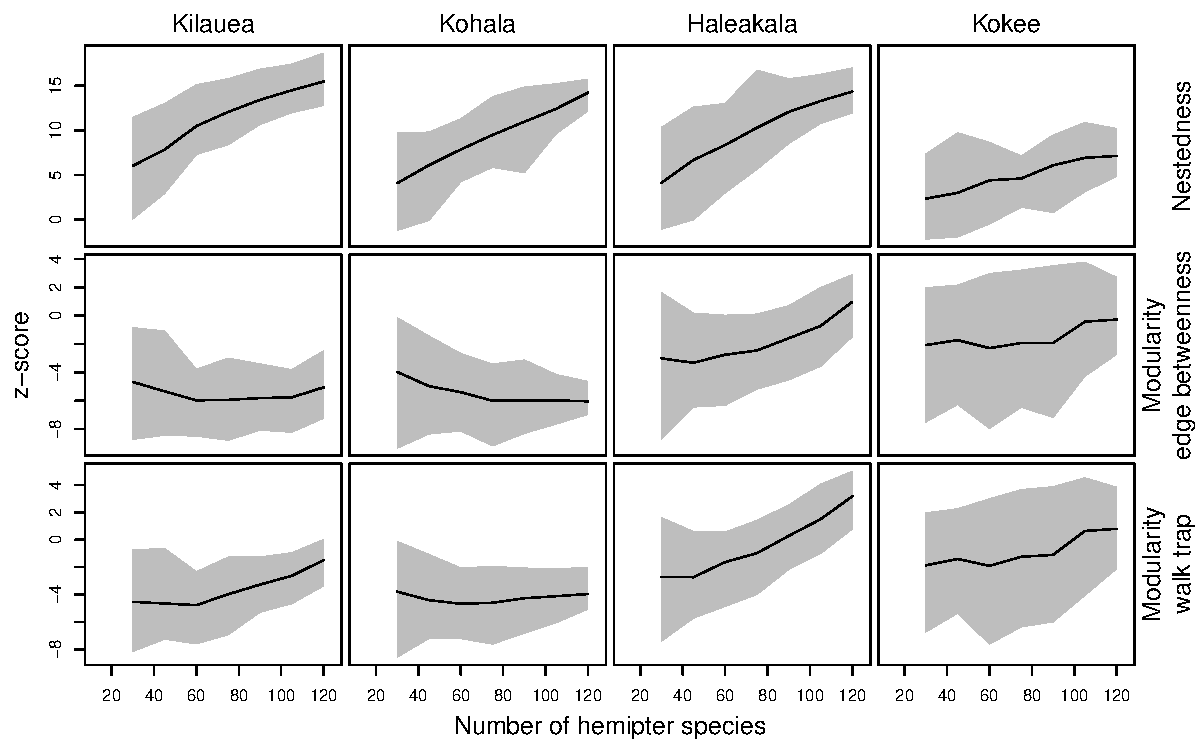
\includegraphics[scale=0.6]{../figSupp_rarified_prob1.pdf}
  \caption{Result from rarification analysis showing sensitivity of
    network metrics to number of Hemiptera sampled.}
  \label{figSupp:rfy}
\end{figure}

\clearpage

\section*{Supplemental Tables}

\begin{table}[!htb]
  \centering
  \begin{tabular}{p{\textwidth}}
    Upon acceptance we will make available our compiled list of
    Hemipitera and their plant hosts from published sources.
  \end{tabular}
  \caption{Published sources of trophic information used to construct networks.}
  \label{tab:networkPubs}
\end{table}


\end{document}




















